\documentclass[aspectratio=169,11pt]{beamer}

\usetheme{Singapore}
\usepackage[utf8]{inputenc}
\usepackage{amsmath}
\usepackage{amsfonts}
\usepackage{amssymb}
\usepackage{graphicx}
\usepackage{hyperref}
\usepackage{booktabs}
\usepackage{listings}
\usepackage{xcolor}
\usepackage{caption}
\usepackage{subcaption}


% Define the settings for codechunks
\definecolor{codegreen}{rgb}{0,0.6,0}
\definecolor{codegray}{rgb}{0.5,0.5,0.5}
\definecolor{codepurple}{rgb}{0.58,0,0.82}
\definecolor{backcolour}{rgb}{0.9,0.9,0.9}
\lstdefinestyle{mystyle}{
    backgroundcolor=\color{backcolour},   
    commentstyle=\color{codegreen},
    keywordstyle=\color{magenta},
    numberstyle=\tiny\color{codegray},
    stringstyle=\color{codepurple},
    basicstyle=\ttfamily\footnotesize,
    breakatwhitespace=false,         
    breaklines=true,                 
    captionpos=b,                    
    keepspaces=true,                 
    numbers=left,                    
    numbersep=5pt,                  
    showspaces=false,                
    showstringspaces=false,
    showtabs=false,                  
    tabsize=2
}
\lstset{style=mystyle}

% Setup the bibliography
\usepackage[style=authortitle,backend=bibtex,citestyle=verbose]{biblatex}
\addbibresource{bibliography.bib}
\setbeamertemplate{bibliography item}[text]
\setbeamerfont{footnote}{size=\tiny}

% Allow footnotes with no number
\newcommand\blfootnote[1]{%
  \begingroup
  \renewcommand\thefootnote{}\footnote{#1}%
  \addtocounter{footnote}{-1}%
  \endgroup
}

% Allow section title slides
\AtBeginSection[]{
  \begin{frame}
  \vfill
  \centering
  \begin{beamercolorbox}[sep=8pt,center,shadow=true,rounded=true]{title}
    \usebeamerfont{title}\insertsectionhead\par%
  \end{beamercolorbox}
  \vfill
  \end{frame}
}

\author{Dr Stephen Pederson}
\title{Lecture 10: Single-Cell RNA Sequencing}
\subtitle{BIOINF3005/7160: Transcriptomics Applications}
%\setbeamercovered{transparent} 
\setbeamertemplate{navigation symbols}{} 
\logo{
	
\includegraphics[scale=0.3]{figures/UoA_logo_col_vert.png} 
} 
\institute{Bioinformatics Hub, \\The University of Adelaide} 
\date{May 25th, 2020} 
\subject{BIOINF3005/7160: Transcriptomics Applications} 


\begin{document}

\begin{frame}
\titlepage
\end{frame}

\begin{frame}
\footnotesize
\tableofcontents
\end{frame}


\section{Background}

\begin{frame}{Introduction}

	\begin{itemize}
		\item scRNA-Seq is the `latest and greatest' transcriptomic technique
		\item Previously all our analysis involved multiple cells per sample
		\begin{itemize}
			\item Now commonly known as bulk RNA-Seq
		\end{itemize}
		\item Large cell numbers during tissue extraction, library preparation etc.
		\item Most experiments have \textbf{highly} heterogeneous cell populations, e.g.
		\pause
		\begin{itemize}
			\item Different regions of the brain contain highly specialised cells
			\item The immune system is highly complex
			\item Cancer samples have both infiltrating and tumour cells
		\end{itemize}
	\end{itemize}


\end{frame}

\begin{frame}{Introduction}

	\begin{itemize}
		\item If a gene is increased 2-fold in expression:
		\begin{itemize}
			\item Is this 2-fold in 100\% of cells?
			\item Or is it 4-fold in 50\% of cells?
			\item Or is it down 2-fold in 25\% and up 8-fold in 25\% and unchanged in 50\%?
		\end{itemize}
		\item Changes in gene expression can be highly specific to individual cell-types
		\item Determining heterogeneity of our bulk samples is challenging
	\end{itemize}

\end{frame}

\begin{frame}{Introduction}

	\begin{itemize}
		\item The most intuitive solution is to obtain RNA from each cell and sequence
		\item Reality is much trickier than this
		\pause
		\item How do we characterise which cell is which cell-type?
		\item What do we even mean by the term `cell-type'?
		\item How do we capture as many transcripts from each cell as we can?
		\begin{itemize}
			\item Missing values are a huge issue in scRNA-seq
		\end{itemize}
		\item How do we compare within the same cell-types between experimental groups?
		\begin{itemize}
			\item e.g. treated and untreated cell types may not be easily assigned to the same cluster/cell-type
		\end{itemize}
	\end{itemize}

\end{frame}


\begin{frame}{Summarised scRNA Workflow}

	\begin{center}
	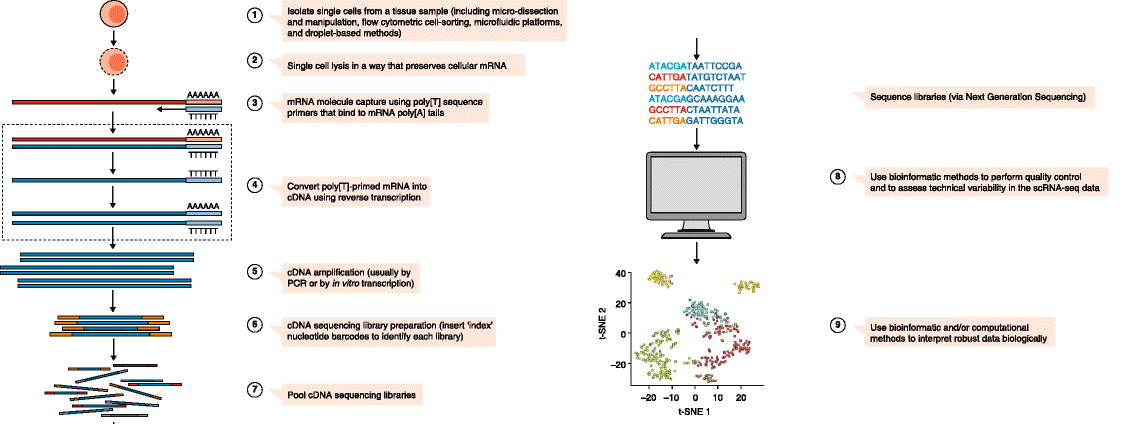
\includegraphics[width=0.9\textwidth]{figures/scRNAWorkflow.png} 
	\end{center}
	
	\blfootnote{Taken from \cite{pmid28821273}}

\end{frame}

\begin{frame}{Motivation}

	\begin{itemize}
		\item Bulk RNA-Seq is primarily focussed on differentially expressed (DE) genes
		\item scRNA-Seq focusses on identifying cell-types within a sample
		\item How do we discriminate between different cell-types and different cell-states?
		\item What is the most intelligent approach for identifying DE genes\\[2mm]
		\begin{itemize}
			\item Is it between clusters/cell-types $\implies$ marker genes
			\item Is it between the same cell-types under differing treatments/cell-states?
		\end{itemize}
	\end{itemize}

\end{frame}

\section{scRNA Protocols}

\begin{frame}{Isolating Individual Cells}

	\begin{itemize}
		\item Early protocols used a dilution series or manual isolation with a microscope (\textit{micromanipulation})
		\item Laser Capture Micro-dissection (LCM)
		\item Fluorescence-Activated Cell Sorting (FACS)
		\begin{itemize}
			\item Labelled antibodies to specific surface markers 
			\item MACS is a magnetic-based approach
		\end{itemize}
		\item Microfluidics/Droplet-based approaches
		\item Multiple rounds of splitting and pooling
	\end{itemize}

\end{frame}

\begin{frame}{Protocol Timeline}

	\begin{center}
		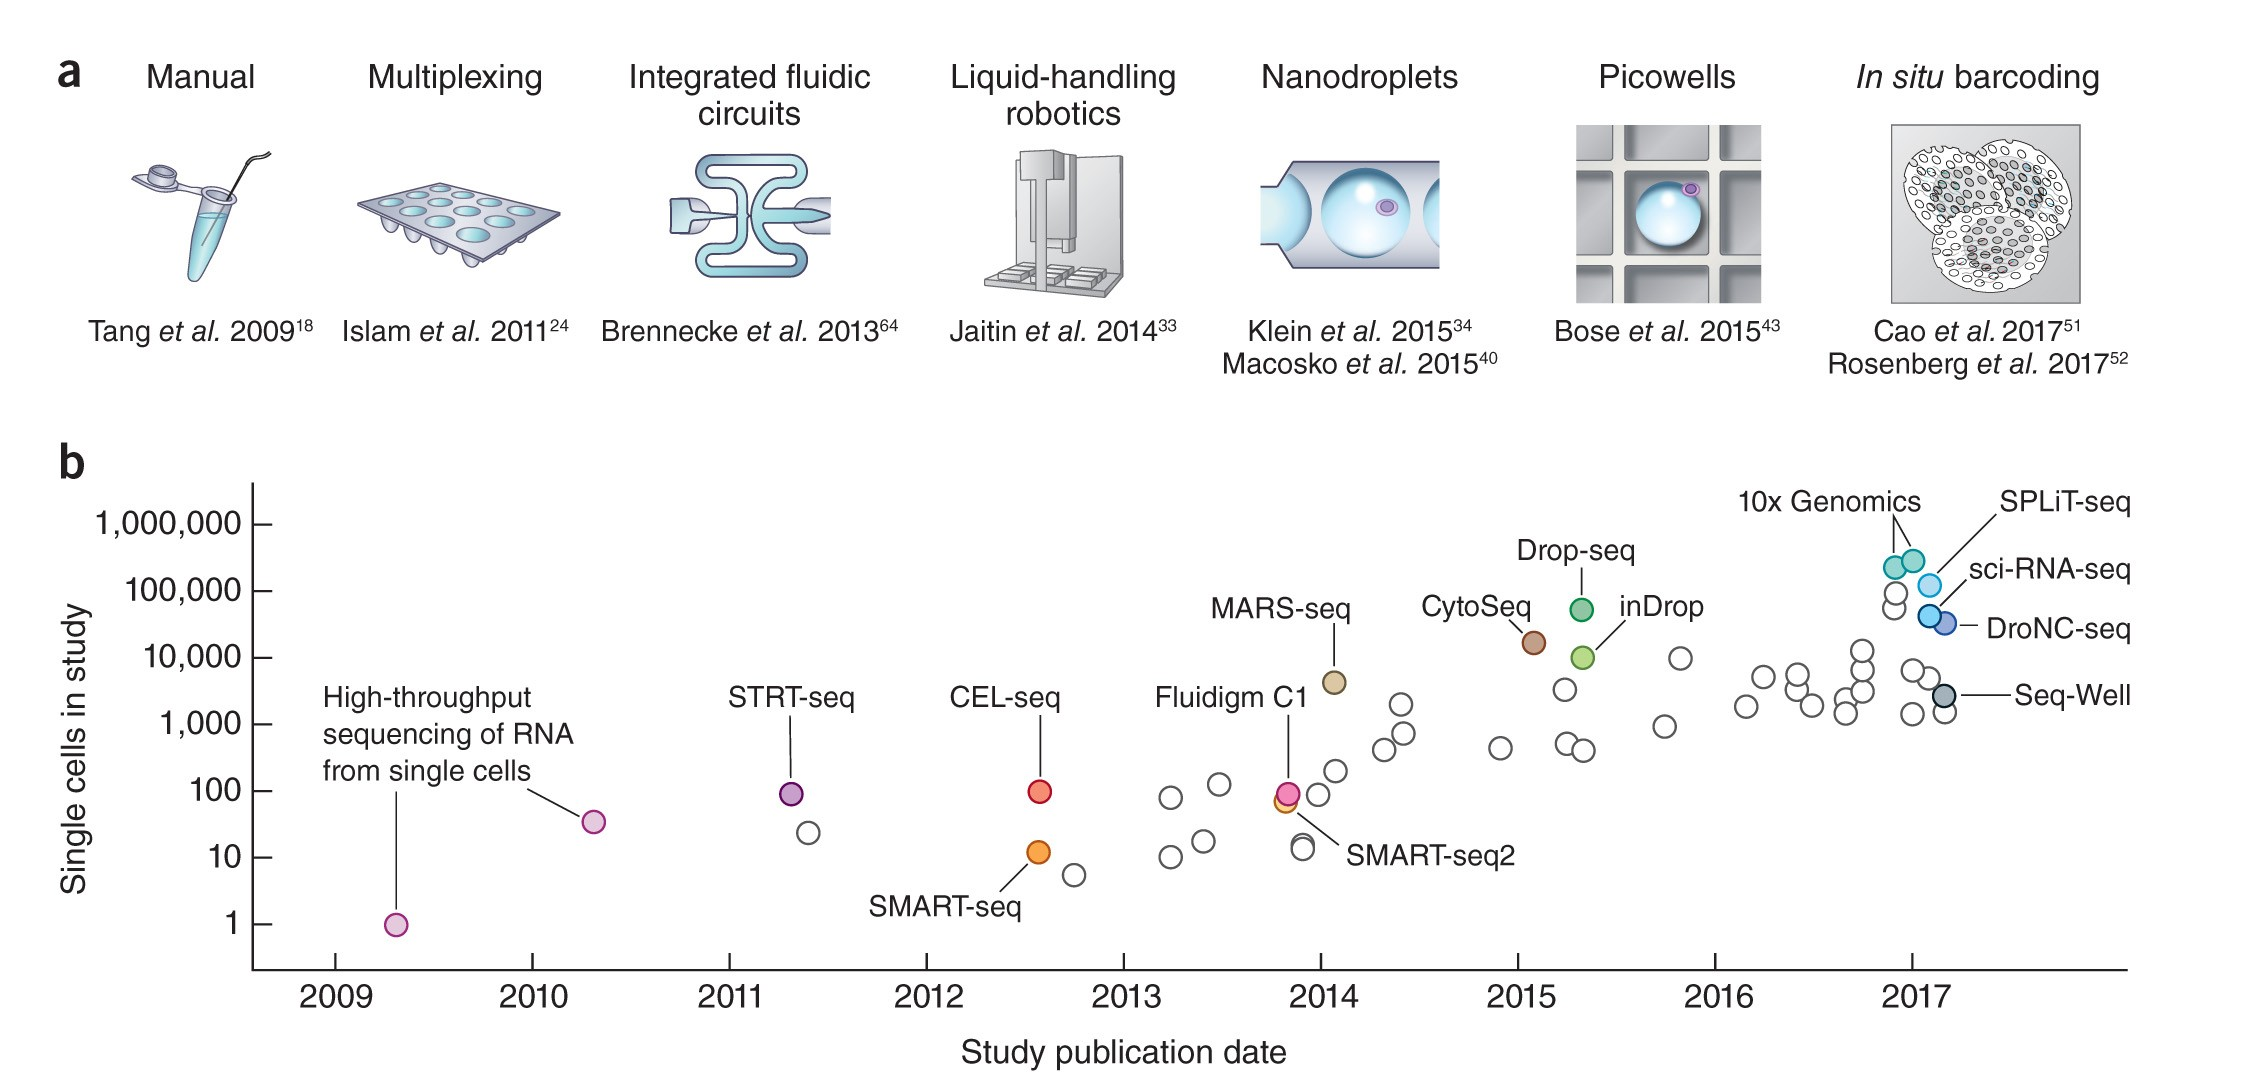
\includegraphics[width=0.85\textwidth]{figures/scRNATimeline.jpg} 
	\end{center}

	\blfootnote{Taken from \cite{pmid29494575}}

\end{frame}

\begin{frame}{Protocol Timeline}

	\begin{center}
		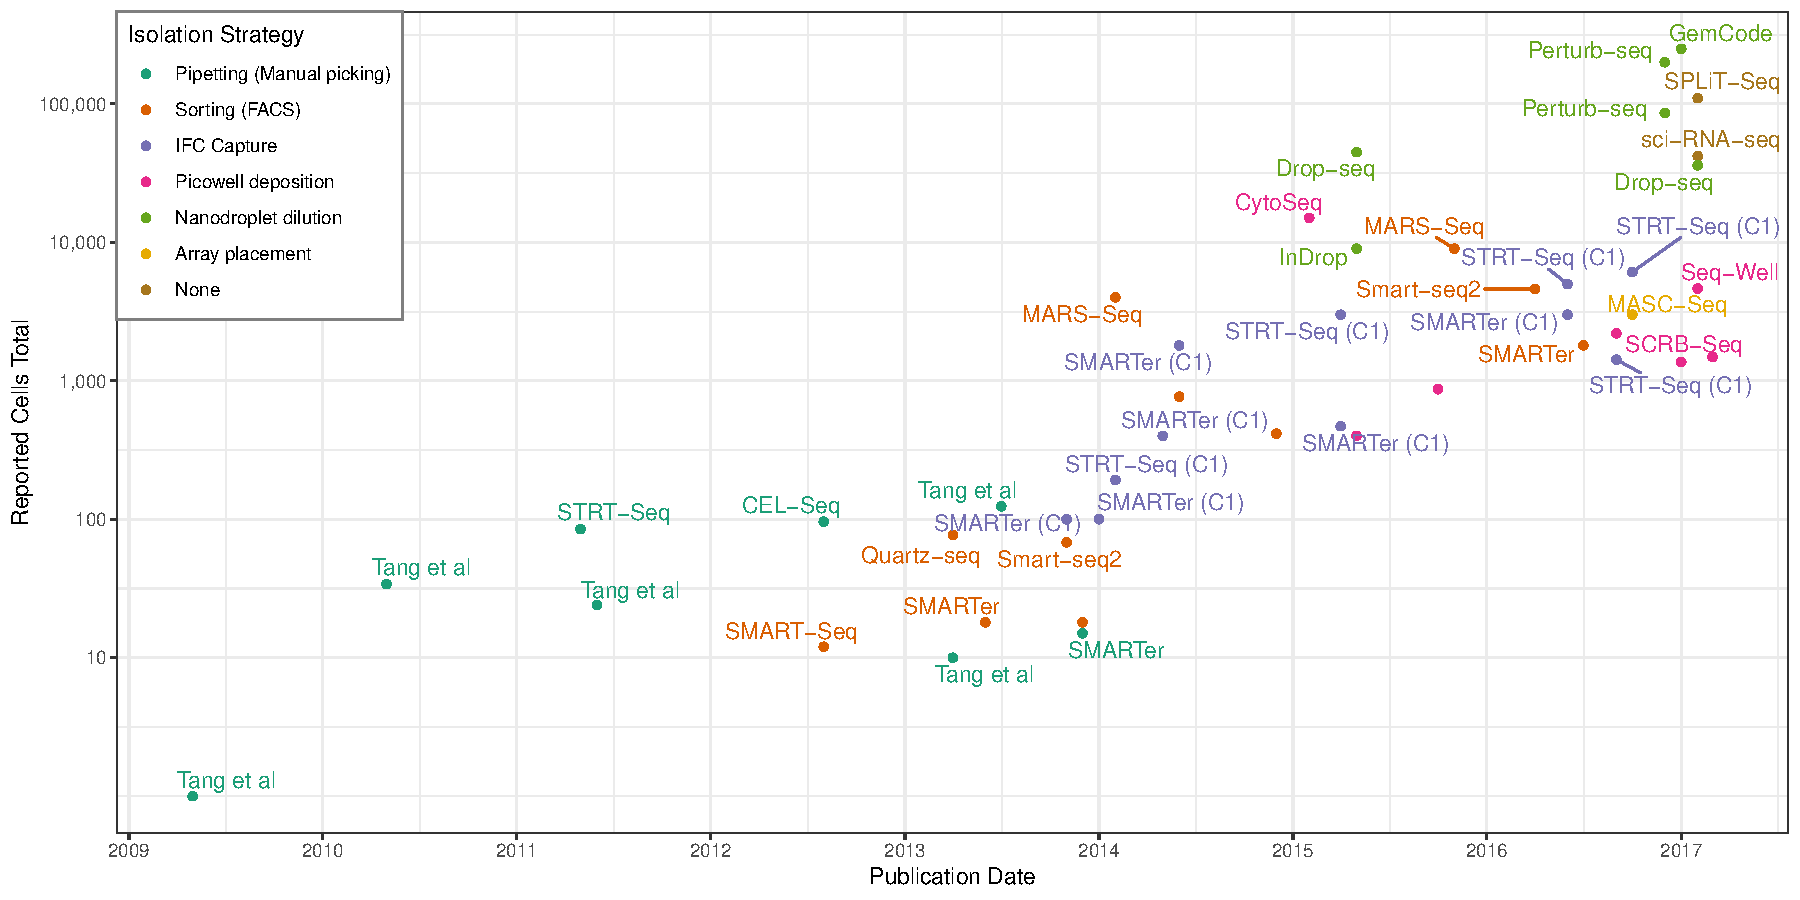
\includegraphics[width=0.85\textwidth]{figures/scRNATimeline.pdf} 
	\end{center}

	\blfootnote{Data taken from \cite{pmid29494575}}

\end{frame}

\begin{frame}{IFC Capture}

	\begin{itemize}
		\item Integrated Fluidic Circuit (IFC) chips
		\begin{itemize}
			\item Most common is the Fluidigm C1
		\end{itemize}
		\item Deliver tiny volumes into `reaction chambers'
		\item Early chips had 96 chambers $\implies$ multiple chips / experiment
		\item Recent chips handle $\sim$800 cells
	\end{itemize}

\end{frame}

\begin{frame}{Protocol Timeline}

	\begin{center}
		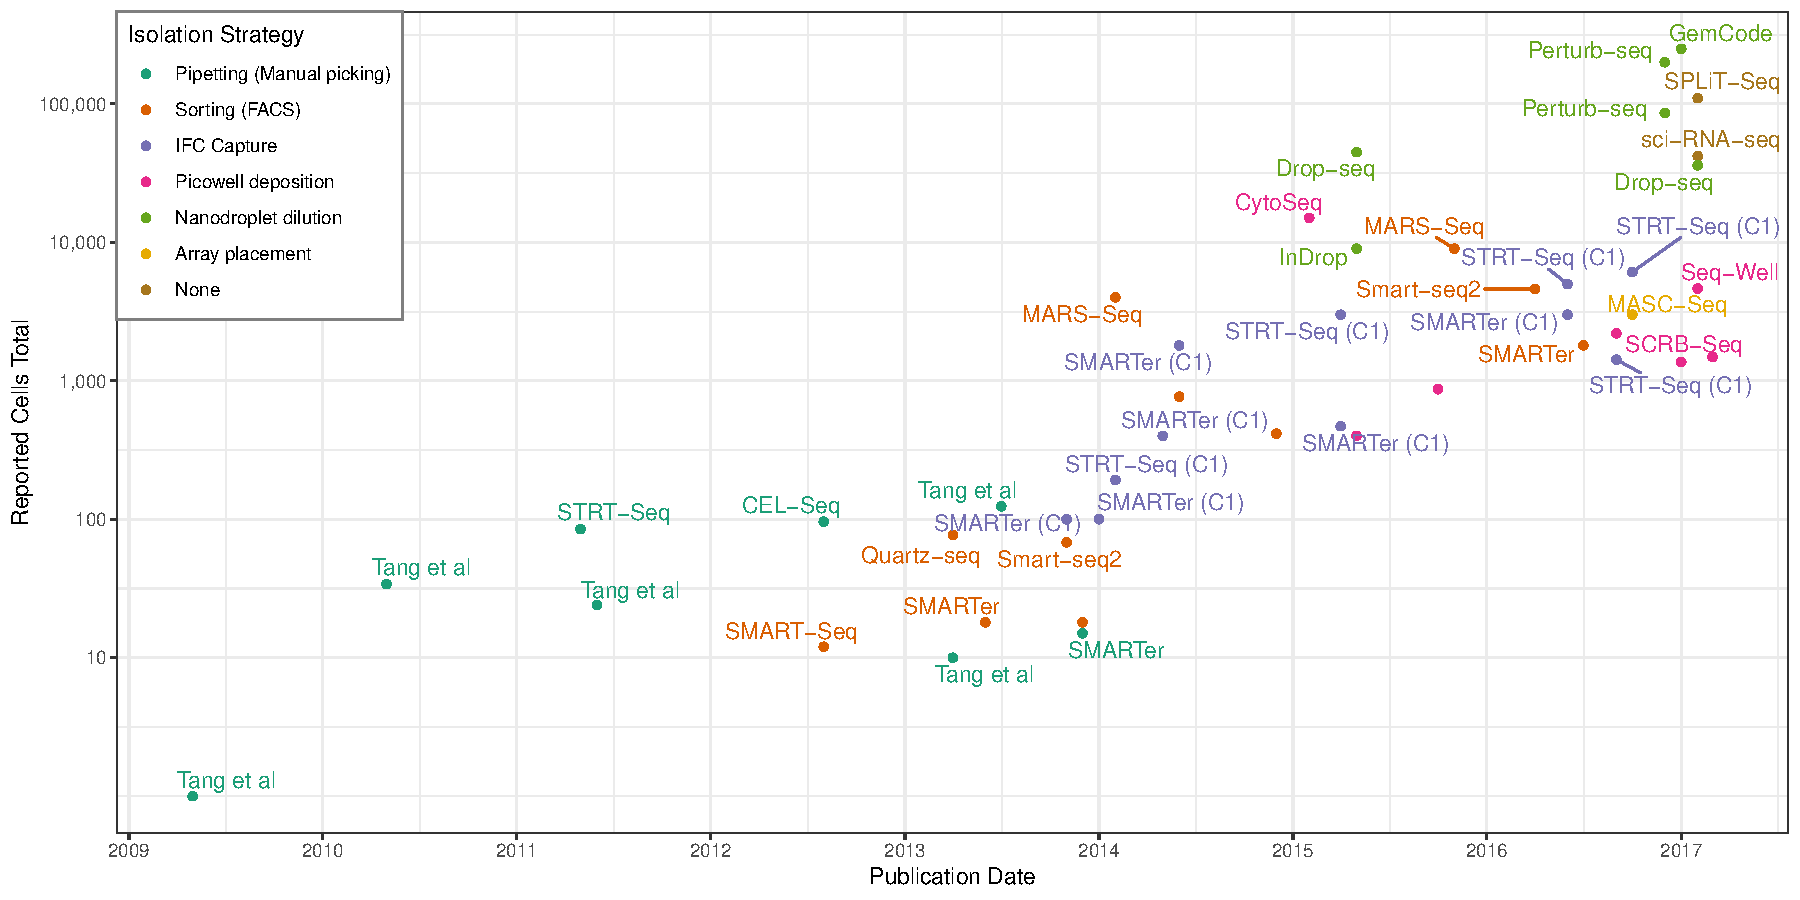
\includegraphics[width=0.85\textwidth]{figures/scRNATimeline.pdf} 
	\end{center}

	\blfootnote{Data taken from \cite{pmid29494575}}

\end{frame}

\begin{frame}{Droplet-based Approaches}

	\begin{center}
		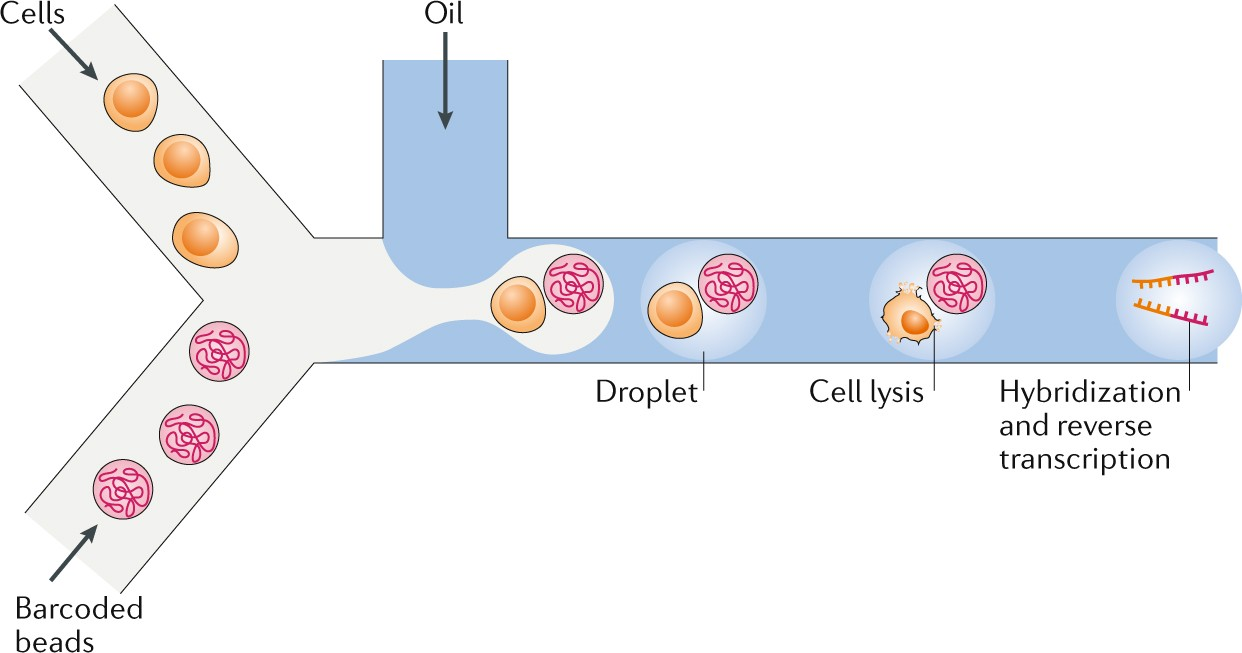
\includegraphics[width=0.7\textwidth]{figures/Droplet.jpg}
	\end{center}
	
	\pause
	Flow rate is modelled as a \textit{Poisson} process to minimise doublets
	
	\blfootnote{Taken from \cite{pmid29789704}}

\end{frame}

\begin{frame}{Sequencing Overview}

	\begin{itemize}
		\item Individual cells are isolated $\implies$ how do we sequence?
		\item Need a method to track which reads come from which cell
		\item Sequencing is performed on a standard Illumina machine, i.e. multiplexed
		\item Each cell is essentially an individual library prep
		\begin{itemize}
			\item Barcodes / UMIs are used for cell / molecule identification
		\end{itemize}
		\item For bulk RNA-Seq we need $0.1-1\mu$g of RNA ($10^5-10^6$pg)
		\begin{itemize}
			\item An individual cell contains 1-50pg RNA
		\end{itemize}
	\end{itemize}

\end{frame}

\begin{frame}{SMART\footnote{SMART = Switching Mechanism at 5' End of RNA Template}-Seq (C1)}

	\begin{enumerate}
		\item All reagents are in the IFC reaction chambers
		\item Cells are lysed
		\item polyA RNA reverse transcribed into \textbf{full length cDNA}
		\begin{itemize}
			\item oligo(dT) priming and template switching
		\end{itemize}
		\item 12-18 PCR cycles
		\item cDNA fragmentation and Adapter ligation
	\end{enumerate}


\end{frame}

\begin{frame}{SMART-Seq (C1)}
	\begin{center}
	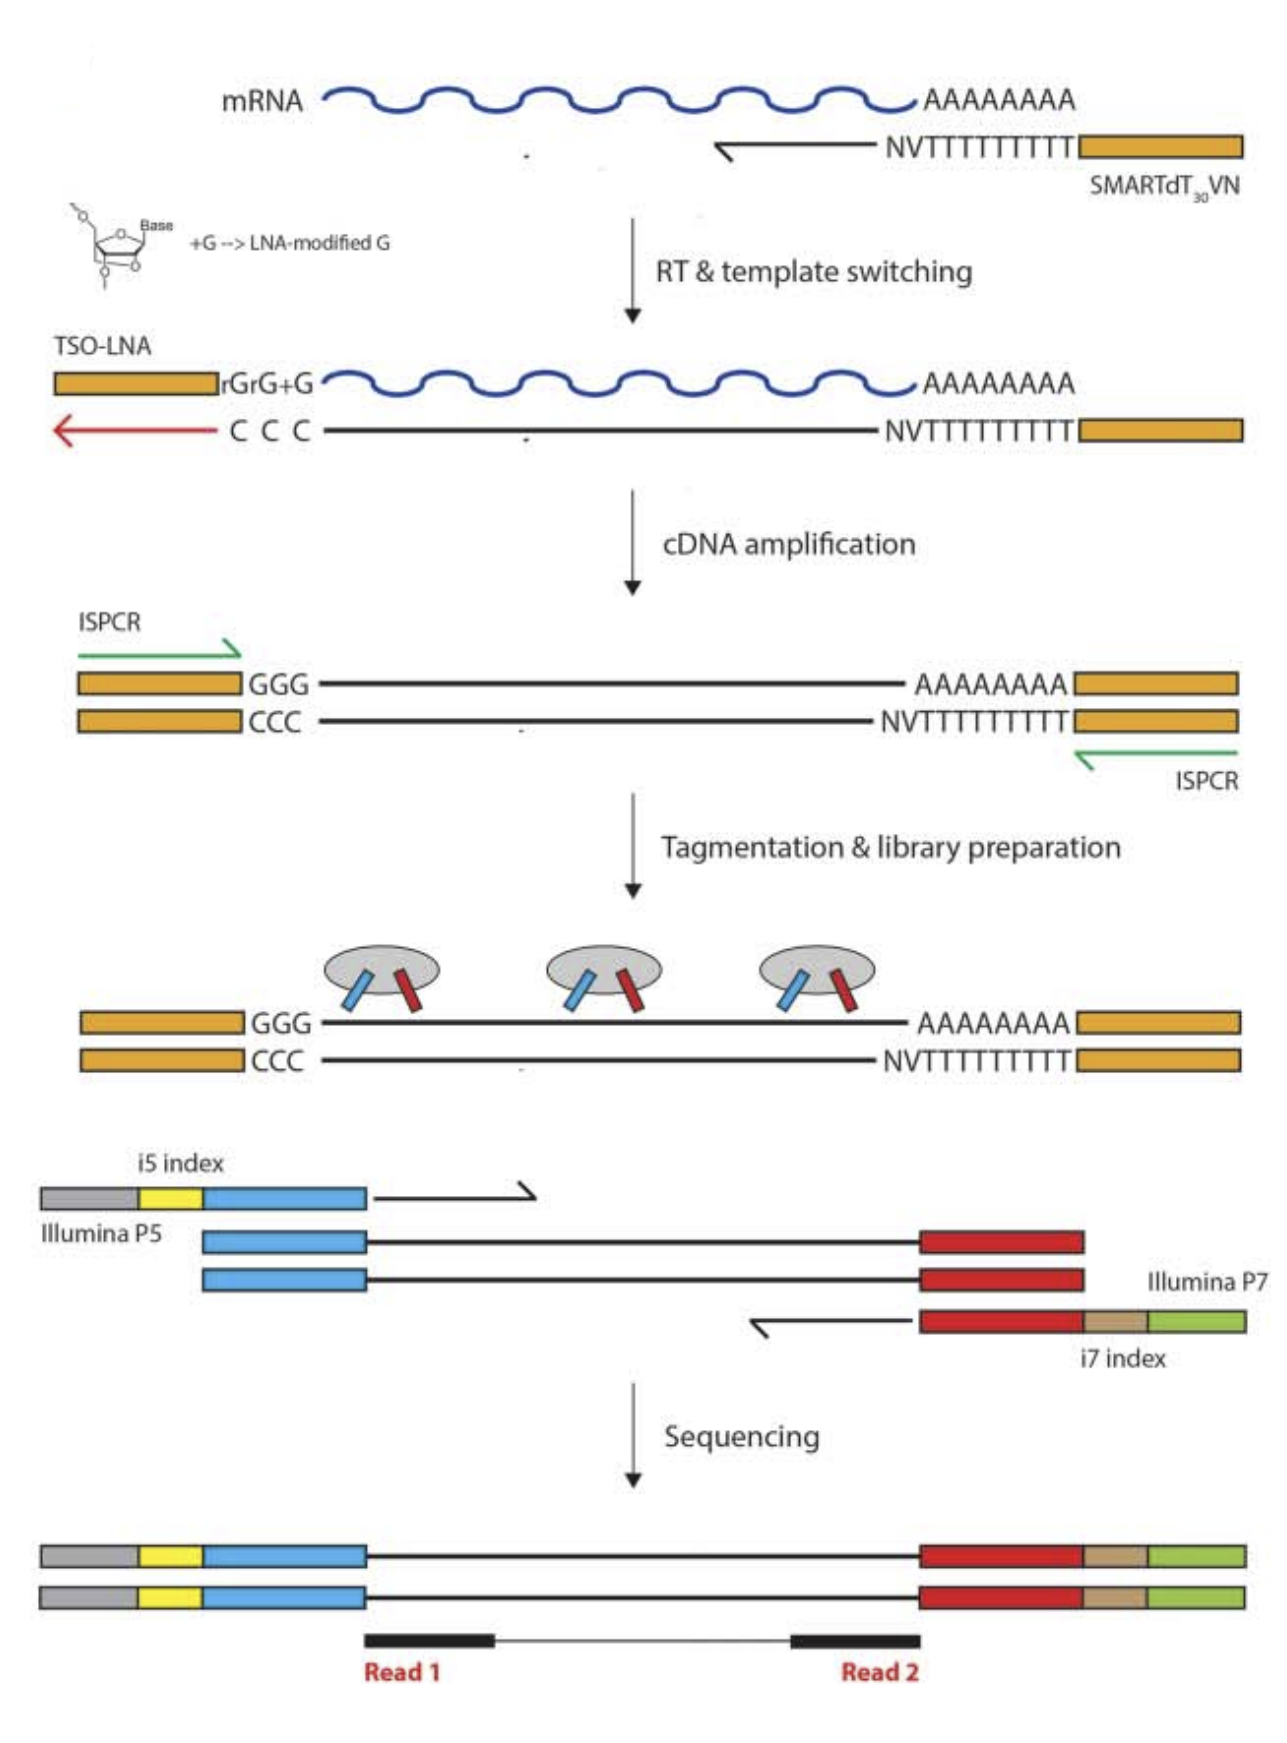
\includegraphics[width=0.3\textwidth]{figures/SMARTSeq.png} 
	\end{center}
	\blfootnote{Image from \cite{pmid27442339}}
\end{frame}

\begin{frame}{Droplet-based Methods}

	\begin{itemize}
		\item Popularised by the 10X Genomics Chromium System
		\item Each gel bead contains the reagents
		\begin{itemize}
			\item 30nt poly(dT) primer with 16nt 10x Barcode, 12nt UMI\footnote{Unique Molecular Identifier}
		\end{itemize}
		\item Illumina primers and restriction enzymes added later
	\end{itemize}

\end{frame}

\begin{frame}{10X Chromium Protocol}

	\begin{columns}[T]
		\begin{column}{.45\textwidth}
			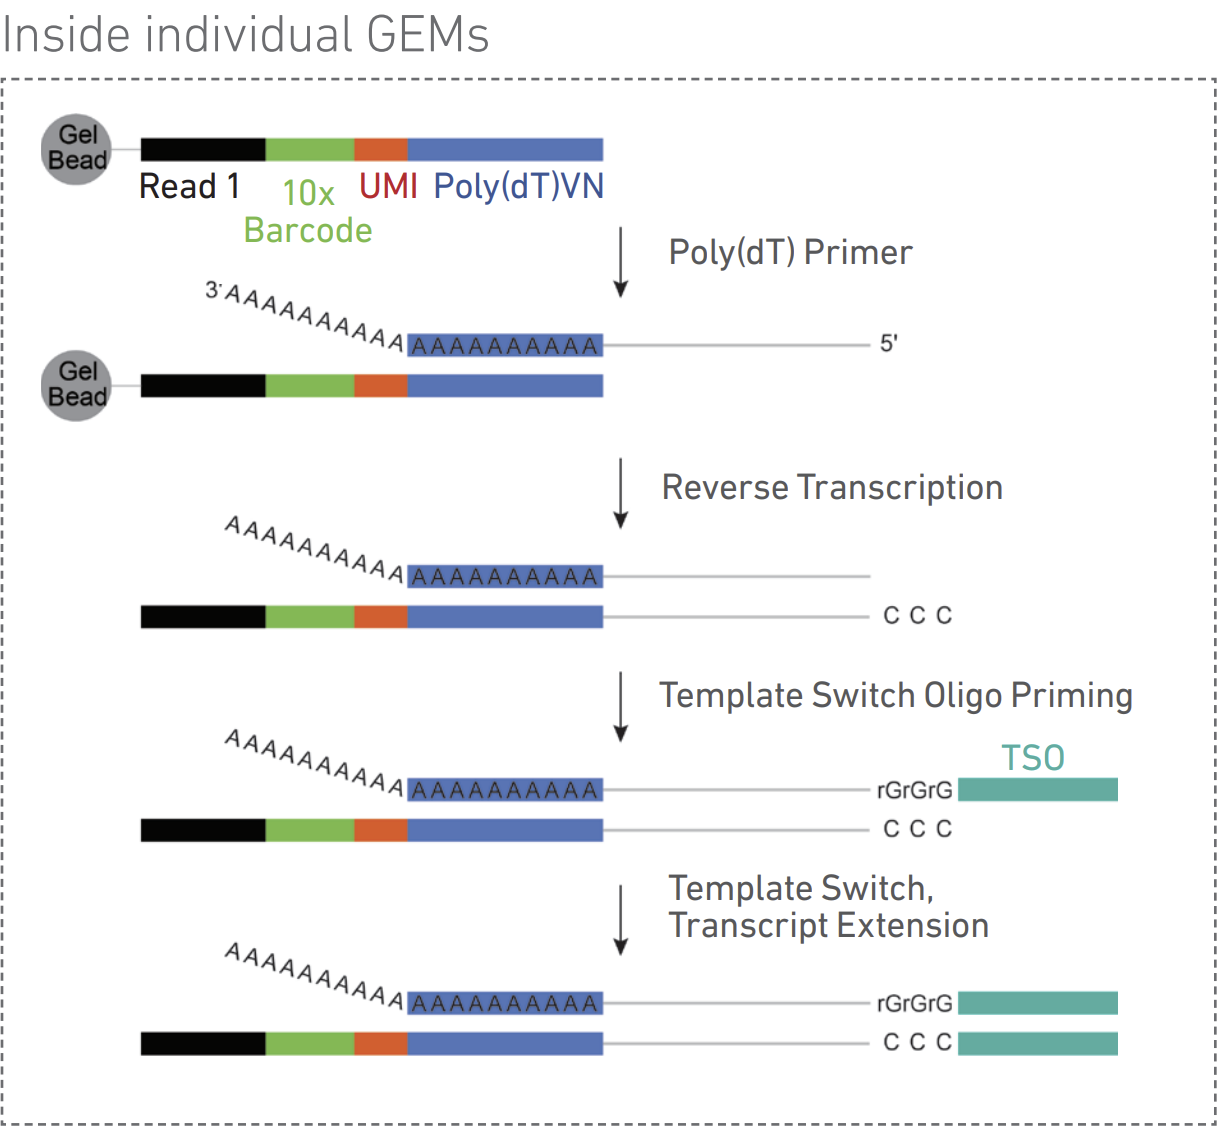
\includegraphics[width=0.75\textwidth]{figures/10xInsideGEM.png} 
			~\\[3mm]
			\small
			Barcoded, full-length cDNA is pooled then PCR amplified
		\end{column}
		\hfill
		\pause
		\begin{column}{.45\textwidth}
			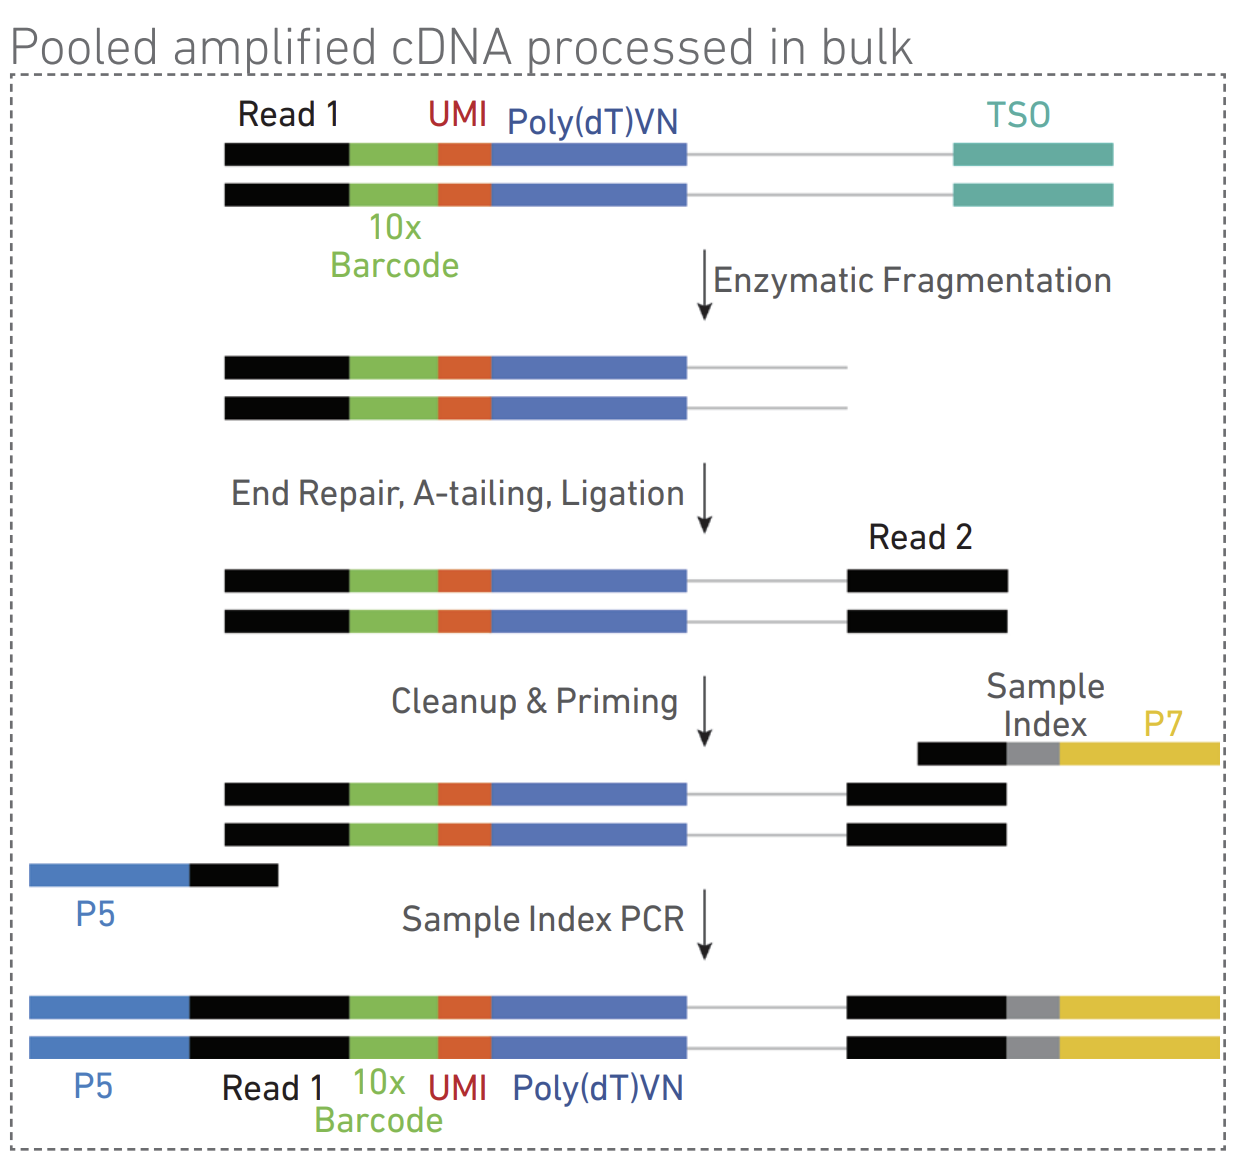
\includegraphics[width=0.75\textwidth]{figures/10xPooled.png} 
		\end{column}
	\end{columns}
	\blfootnote{Images from \href{https://assets.ctfassets.net/an68im79xiti/1eX2FPdpeCgnCJtw4fj9Hx/7cb84edaa9eca04b607f9193162994de/CG000204\_ChromiumNextGEMSingleCell3\_v3.1\_Rev\_D.pdf}{10X Genomics CG000204\_ChromiumNextGEMSingleCell3\_v3.1\_Rev\_D.pdf}}
\end{frame}

\begin{frame}{10X Chromium Protocol}
	\begin{center}
		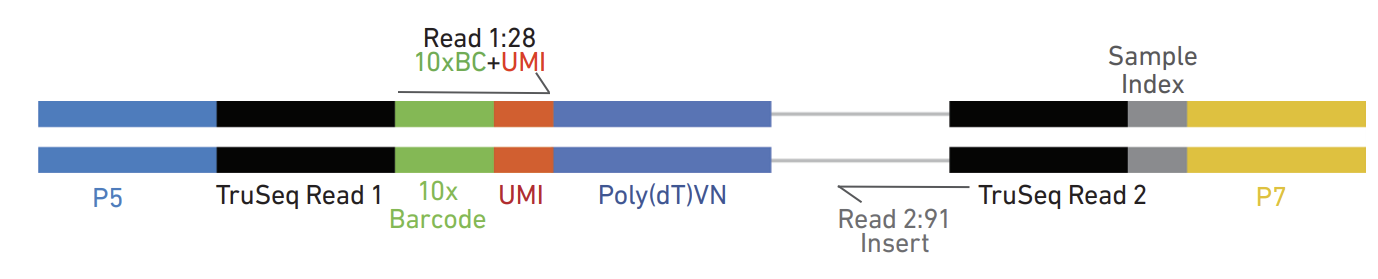
\includegraphics[width=0.6\textwidth]{figures/10XPairedRead.png} 
	\end{center}
	
	\begin{itemize}
		\item Only R2 contains the sequence information
		\item Only the 3' end is sequenced
		\item Each template RNA should have one UMI $\implies$ PCR duplicates can be identified
	\end{itemize}		
	
\end{frame}

\begin{frame}{Other Variations}

CITE-Seq\footnote{Cellular Indexing of Transcriptomes and Epitopes by sequencing}
	
	\begin{itemize}
		\item Prior to sorting cells can be `labelled' with antibody-oligo complexes
		\item Oligos allow additional recognition of surface proteins
		\item On cell lysis these oligos are amplified along with RNA
	\end{itemize}		
	
\end{frame}

\begin{frame}{Other Variations}

SPLIT-Seq\footnote{Split-Pool Ligation-based Transcriptome Sequencing}
	\begin{itemize}
		\item Cells are split into pools and fixed
		\item One barcode/pool
		\item Multiple rounds of pooling and barcoding
		\item All amplification is \textit{in situ}
		\item Able to be applied to single nuclei
	\end{itemize}
	
\end{frame}

\begin{frame}{Comparison of Methods}

	\begin{center}
	
		\small
		\begin{tabular}{l|llll}
			\textbf{Protocol} & \textbf{C1 (SMART-Seq)} & \textbf{SMART-Seq2} & \textbf{10X Chromium} & \textbf{SPLIT-Seq}\\
			\midrule
			\textit{Platform} & Microfluidics & Plate-based & Droplet & Plate-based\\
			\textit{Transcript} & Full-length & Full-length & 3'-end & 3'-end\\
			\textit{Cells} & $10^2 - 10^3$ & $10^2 - 10^3$ & $10^3-10^4$ & $10^3 - 10^5$\\
			\textit{Reads/Cell} & $10^6$ & $10^6$ & $10^4-10^5$ & $10^4$\\
			\bottomrule
		\end{tabular}

	\end{center}
	\pause
	~\\[3mm]
	Saturation for detection of expressed genes occurs around $5\times10^5$ reads/cell

	\blfootnote{Data sourced from \cite{pmid28821273}}

\end{frame}

\begin{frame}{Protocol Timeline}

	\begin{center}
		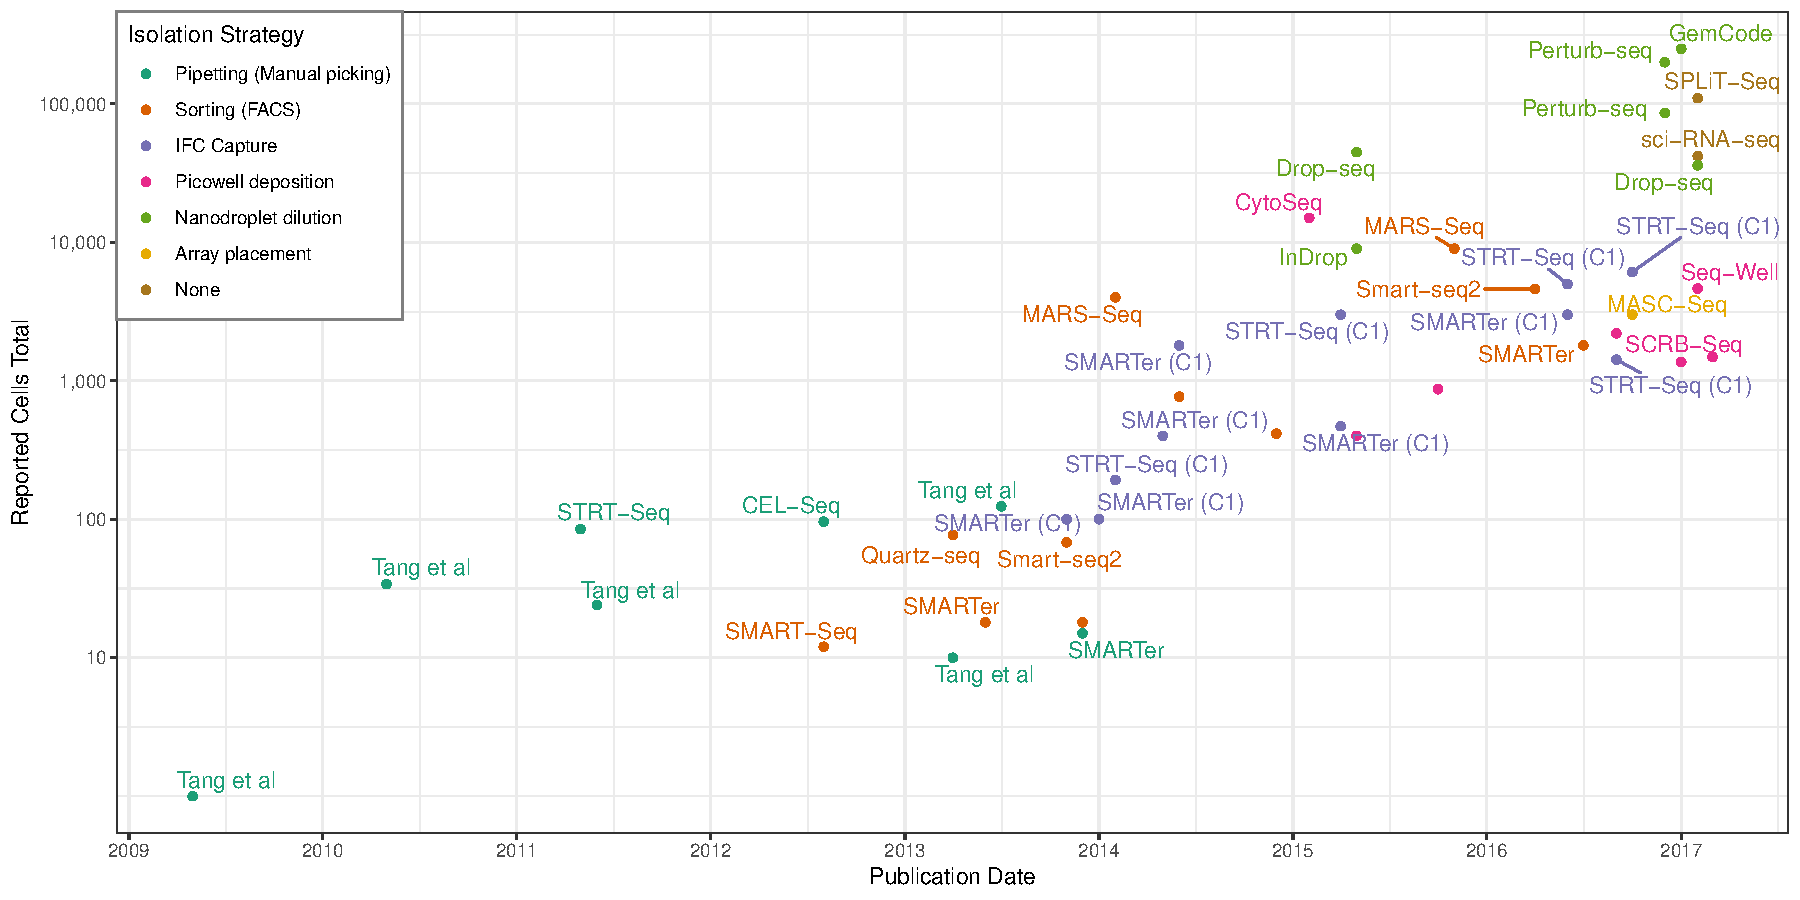
\includegraphics[width=0.85\textwidth]{figures/scRNATimeline.pdf} 
	\end{center}

	\blfootnote{Data taken from \cite{pmid29494575}}

\end{frame}

\begin{frame}{Technical Challenges}

	\begin{itemize}
		\item How to detect intact/viable cells, free RNA etc
		\item How to ensure only single cells captured, i.e. no doublets
		\item Unbiased of sampling of RNA molecules (e.g. PCR impacts) and individual cells
		\begin{itemize}
			\item Large numbers of zero counts for expressed genes
			\item Lack of evidence for expression $\neq$ evidence for lack of expression
		\end{itemize}
		\item Efficiency of cell capture ($\sim$50\% for 10X)
		\item How to deal with batch effects
		\begin{itemize}
			\item Cells from each treatment group are always prepared separately
		\end{itemize}
	\end{itemize}

\end{frame}

\section{Data Analysis}

\begin{frame}{Automated Pipelines}
	\begin{itemize}
		\item Most pre-processing for 10X data is performed using \texttt{CellRanger}
		\item Handles demultiplexing, alignment (\texttt{STAR}) and quantification (using UMIs)
		\begin{itemize}
			\item Full-length transcript methods can utilise \texttt{kallisto/salmon}
		\end{itemize}
		\item We end up with a \texttt{feature-barcode matrix}
		\begin{itemize}
			\item A \textbf{barcode} represents an individual cell (or a set of reactions)
			\item A \textbf{feature} is commonly thought of as a gene in scRNA-Seq
			\item Other single-cell approaches (e.g. scATAC-Seq) are not gene focussed
		\end{itemize}
		\item Similar to counts from bulk RNA-Seq but with many more columns (cells)
	\end{itemize}
\end{frame}

\begin{frame}{Filtering}

	\begin{itemize}
		\item We need to keep the high quality cells and discard the dubious cells, such as:\\[2mm]
		\begin{enumerate}
			\item Low/High read numbers (library sizes)
			\item Low feature/gene numbers
			\item High proportions of mitochondrial RNA $\implies$ cells broken prior to lysis\\[2mm]
		\end{enumerate}
		\pause
		\item Also need a method for considering each gene as detectable (Average Counts $>1$)
		\begin{itemize}
			\item Treatment Groups and Cell-Types are less easily defined \textit{a priori}
		\end{itemize}
	\end{itemize}

\end{frame}


\begin{frame}{Normalisation}
	\begin{itemize}
		\item Cell-specific offsets are once again calculated
		\begin{itemize}
			\item Each cell is it's own source of variability
		\end{itemize}
		\item Methods such as TMM are heavily influenced by the large numbers of zero counts
		\item Pooling and deconvolution:
		\begin{enumerate}
			\item Perform rudimentary clustering of cells		
			\item Normalise across all clusters (TMM assumes most genes are not DE)
			\item Deconvolute cells and normalisation factors
		\end{enumerate}
		\item Calculate log-transformed, normalised expression values (\texttt{logcounts})
	\end{itemize}
\end{frame}

\begin{frame}{Clustering}

	\begin{itemize}
		\item A key process is grouping similar cells with each other $\implies$ identifying cell-types
		\item To speed this up, we often choose the most highly variable genes (HVGs)
		\item Perform dimensional reduction:
		\begin{itemize}
			\item PCA is the preferred linear approach, with non-linear approaches being:
			\item tSNE (t-Distributed Stochastic Neighbour Embedding)
			\item UMAP (Uniform Manifold Approximation and Projection)
		\end{itemize}
		\item Both tSNE and UMAP are highly sensitive to parameter choice
	\end{itemize}

\end{frame}

\begin{frame}{Clustering}

	\begin{columns}[T]
		\begin{column}{.45\textwidth}
			\centering
			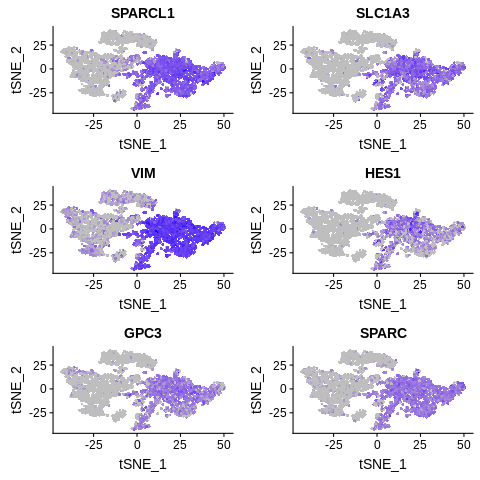
\includegraphics[width=0.75\textwidth]{figures/eCRfeatureplotmarker.png} 
		\end{column}
		\hfill
		\begin{column}{.45\textwidth}
			\centering
			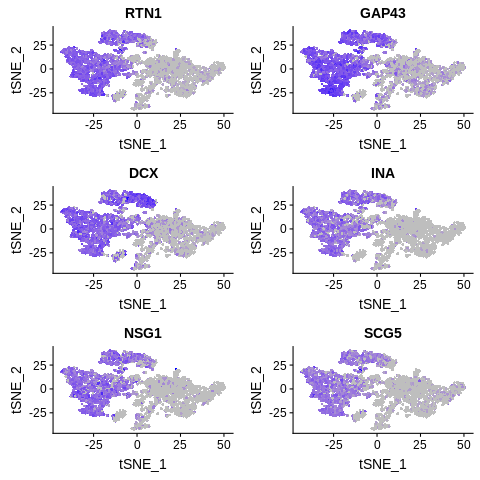
\includegraphics[width=0.75\textwidth]{figures/eCRfeatureplotpca.png} 
		\end{column}
	\end{columns}
	\blfootnote{Images from \url{https://scrnaseq.readthedocs.io/en/latest/ecellranger.html}}
	
\end{frame}

\begin{frame}{Clustering}

	\begin{itemize}
		\item Formation of clusters allows for \textit{identification of cell-types}
		\item Is there a ``ground truth"?
		\item Different approaches will provide different results
		\item Different parameter settings with provide different results
		\item Each approach could be considered an alternate view-point on the data
		\begin{itemize}
			\item Some viewpoints reveal particular information
			\item Alternate viewpoints reveal different insights
		\end{itemize}
		\item These are not necessarily contradictory
		\item Clusters are essentially \textit{artificial constructs} used to represent one or more biological features
	\end{itemize}
	
\end{frame}

\begin{frame}{Graph-Based Clustering}

	\begin{itemize}
		\item Common approaches are $k$-nearest neighbours / shared neighbour weighting
		\item Relatively efficient computationally
		\item Uses the reduced dimensional data \textbf{not gene expression}
		\begin{itemize}
			\item Commonly PCA with some optimising for the number of retained PCs
		\end{itemize}
		\item Represents the similarity between cells as an ``edge weight" 
		\item No assumption about `shape' of any clustering
		\item Clusters are identified using \textit{Community Detection}
	\end{itemize}

\end{frame}

\begin{frame}{Visualising Clusters: tSNE}

	\begin{center}
	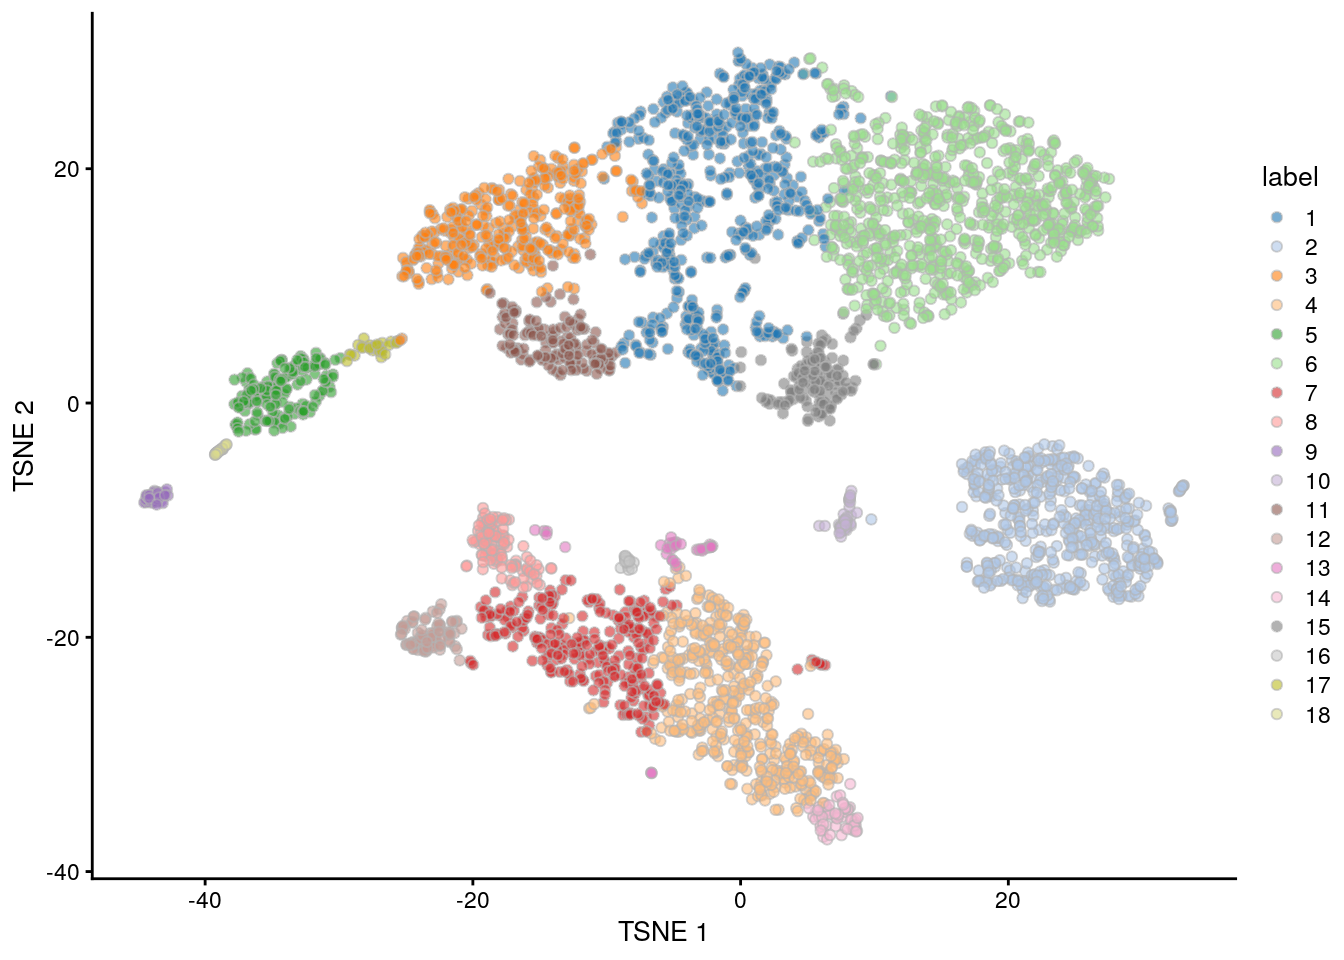
\includegraphics[width=0.6\textwidth]{figures/tsne-clust-graph-1.png} 
	\end{center}
	
	\blfootnote{Image taken from \href{https://osca.bioconductor.org/}{Orchestrating Single-Cell Analysis with Bioconductor}}
	
\end{frame}

\begin{frame}{Visualising Clusters: Force-Directed Layout}

	\begin{center}
	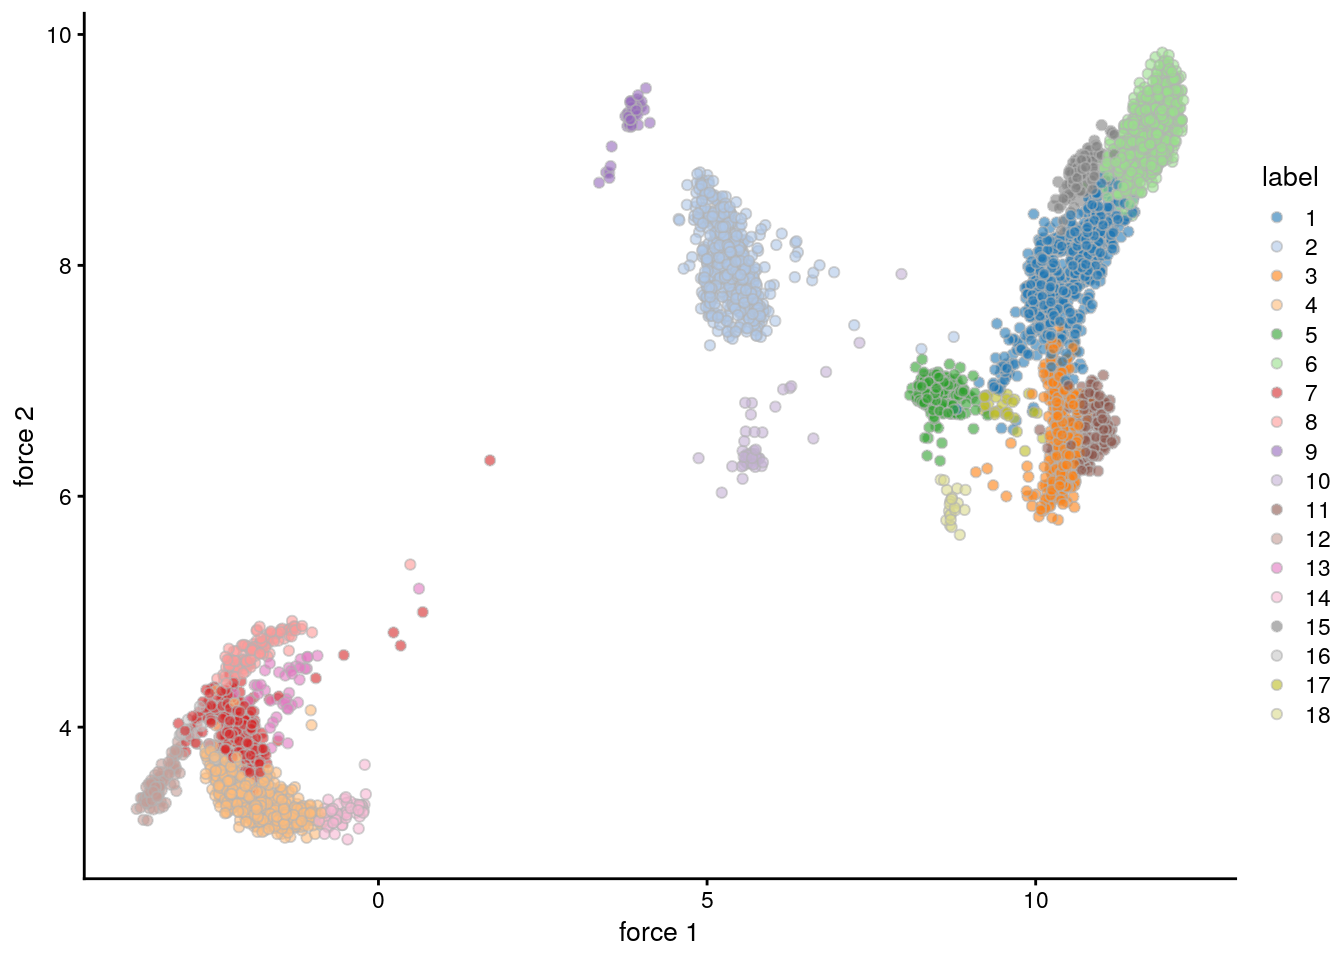
\includegraphics[width=0.6\textwidth]{figures/pbmc-force-1.png} 
	\end{center}
	
	\blfootnote{Image taken from \href{https://osca.bioconductor.org/}{Orchestrating Single-Cell Analysis with Bioconductor}}
	
\end{frame}

\begin{frame}{Graph-Based Clustering}

	\begin{itemize}
		\item Forcing a minimum number of neighbours minimises small clusters
		\begin{itemize}
			\item Choosing large $k$ gives fewer larger clusters
		\end{itemize}
		\item Clustering is performed in high-dimensions (e.g. using 10PCs) but visualised in 2
		\item Is essentially an exploratory process
	\end{itemize}
	
\end{frame}

\begin{frame}{Graph-Based Clustering}

	\begin{center}
		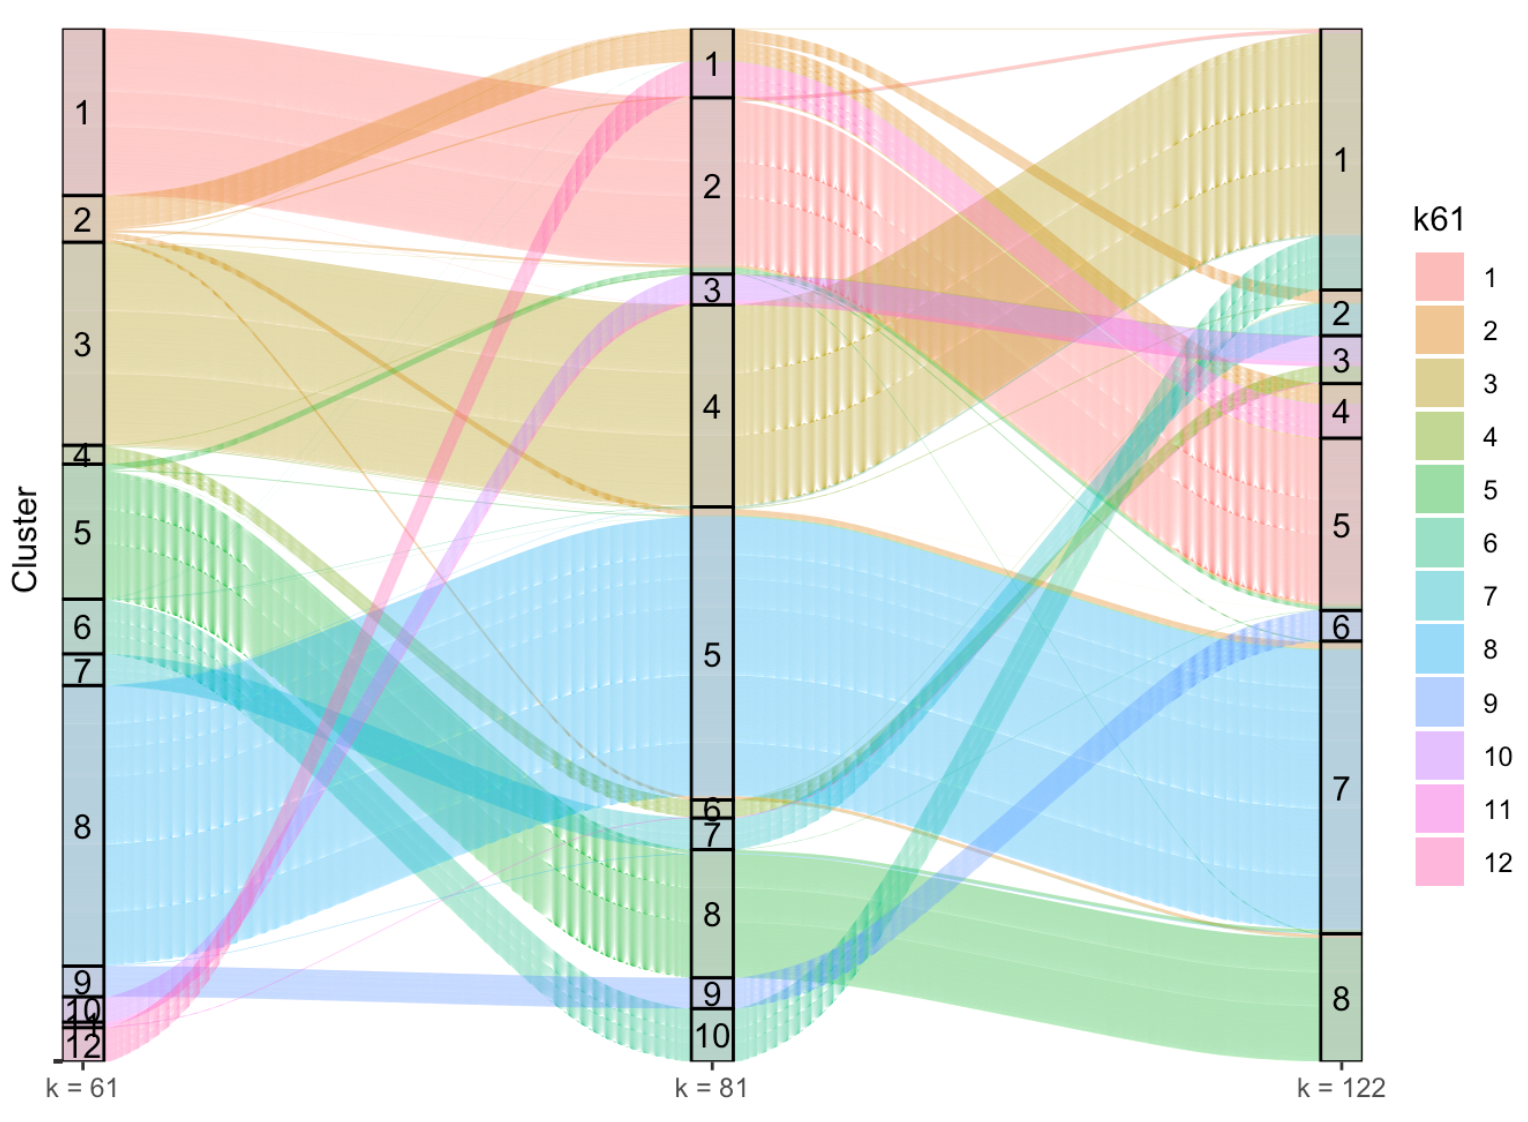
\includegraphics[width=0.55\textwidth]{figures/junweiAlluvial.png} 
	\end{center}
	
	\blfootnote{Image from Junwei Wang, Masters Thesis, 2019}

\end{frame}

\begin{frame}{Alternative Clustering Methods}
	\begin{itemize}
		\item We can use $k$-Means $\implies$ assumes $k$ multi-dimensional spheres
		\item $k$ explicitly sets the number of clusters
	\end{itemize}
	
\end{frame}

\begin{frame}{Alternative Clustering Methods}
	\begin{columns}[T]
		\begin{column}{.45\textwidth}
			\centering
			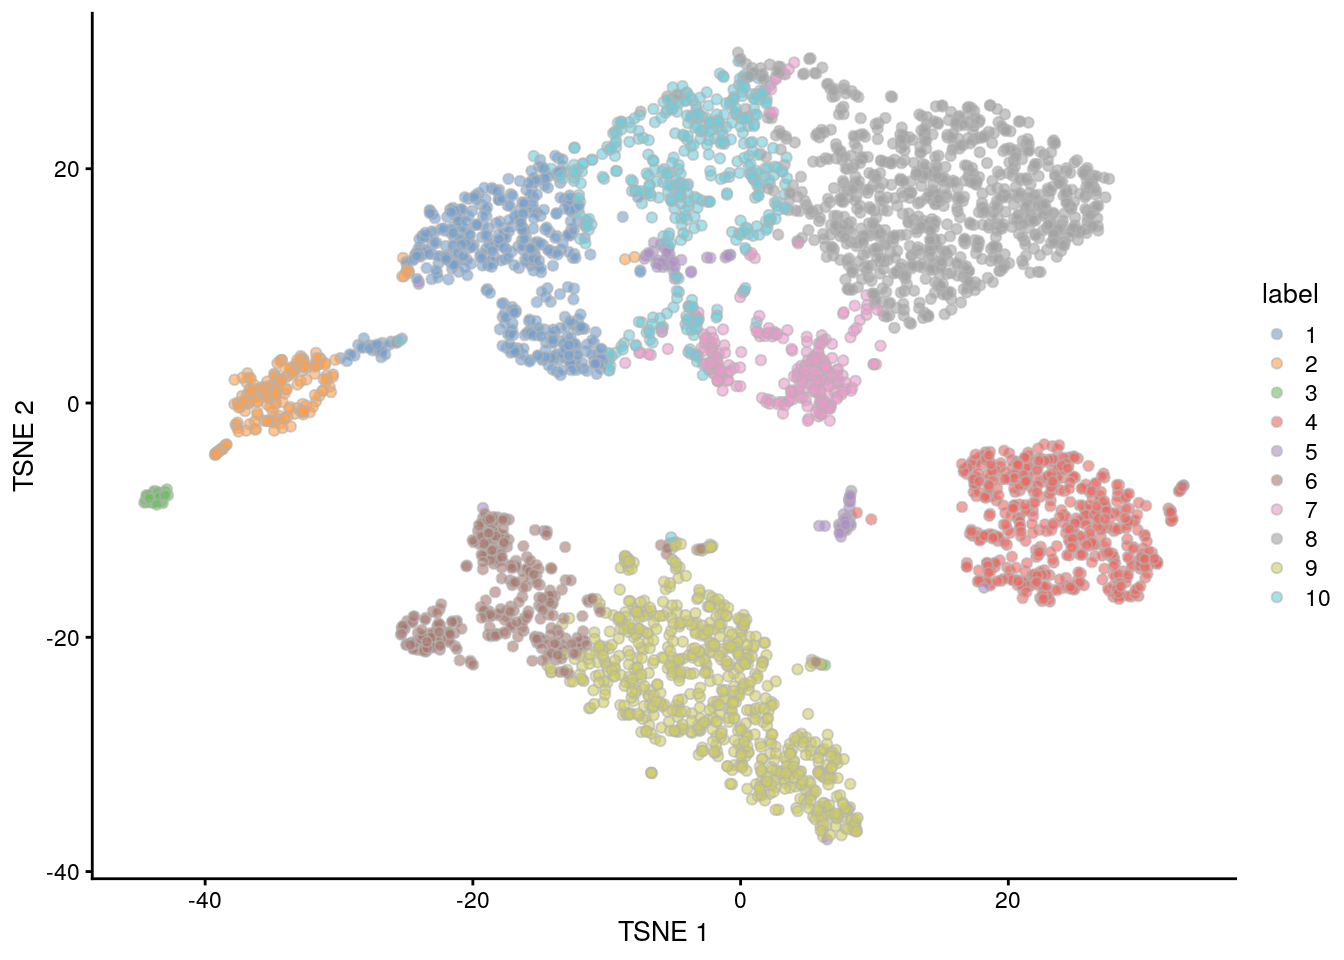
\includegraphics[width=0.95\textwidth]{figures/tsne-clust-kmeans-1.png} 
			~\\
			Setting $k = 10$
		\end{column}
		\hfill
		\pause
		\begin{column}{.45\textwidth}
			\centering
			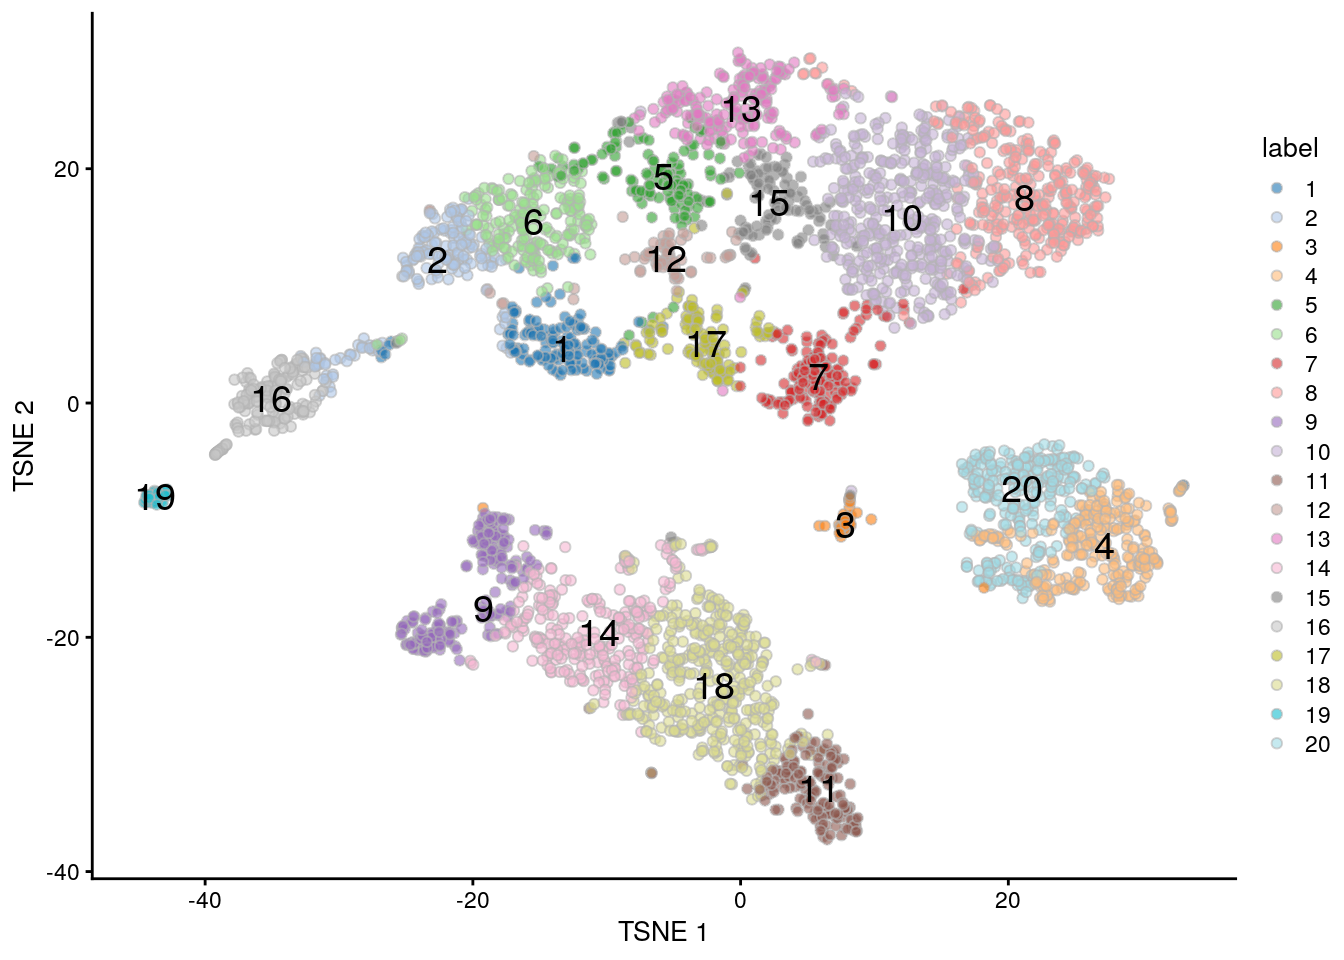
\includegraphics[width=0.95\textwidth]{figures/tsne-clust-kmeans-best-1.png} 
			~\\
			Setting $k=20$
		\end{column}
	\end{columns}
	\blfootnote{Images taken from \href{https://osca.bioconductor.org/}{Orchestrating Single-Cell Analysis with Bioconductor}}
\end{frame}


\begin{frame}{Marker Selection}

	\begin{itemize}
		\item An alternative perspective to differential expression $\implies$ marker gene selection
		\item We find which genes \textit{define} one or more clusters $\implies$ identify known/unknown cell types
		\item Can also use known markers from CITE-Seq to identify cell-types
		\item Each cluster needs to be compared to all other clusters
		\begin{itemize}
			\item Can use $t$-tests, \texttt{limma/voom}, \texttt{edgeR}
			\item For unique markers, choose the maximal p-value across all comparisons
		\end{itemize}
	\end{itemize}

\end{frame}

\begin{frame}{Marker Selection}

	\begin{center}
		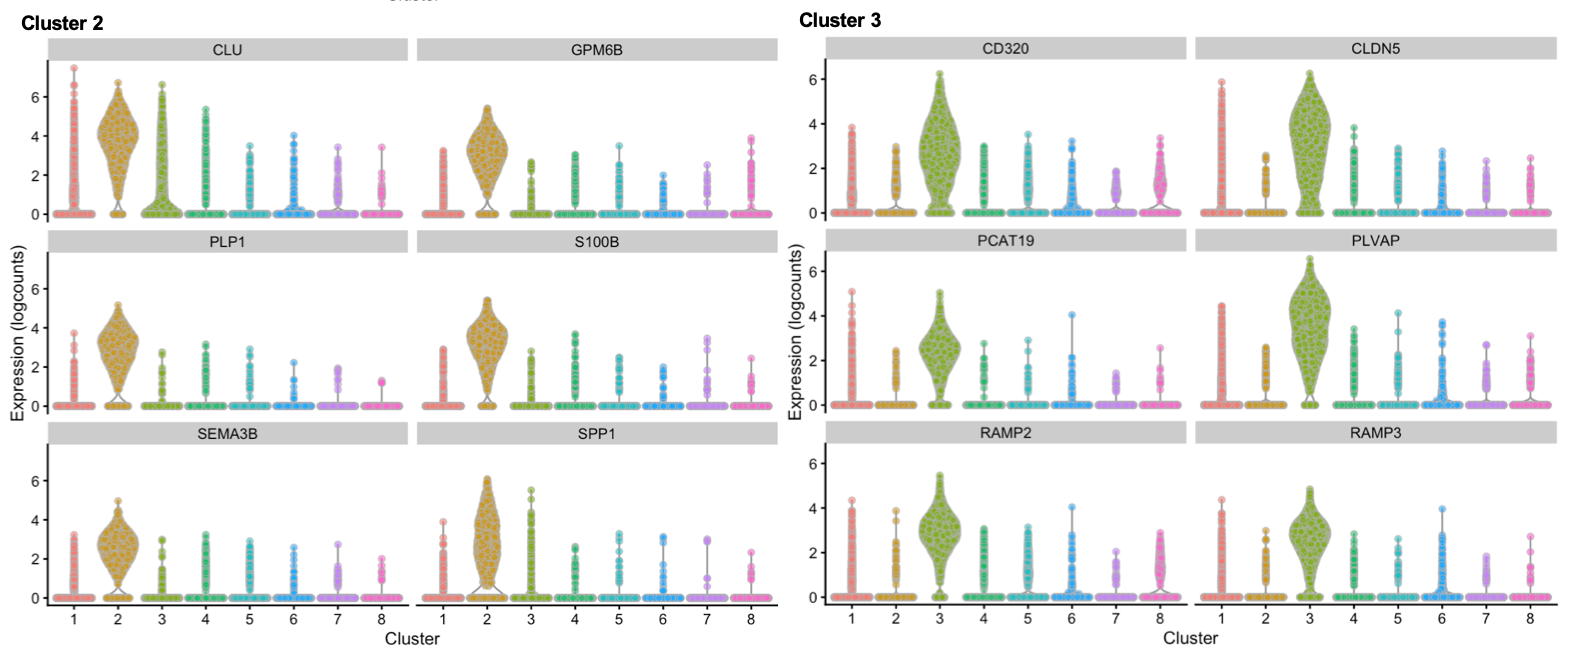
\includegraphics[width=0.9\textwidth]{figures/junweiCluster3.png}
	\end{center}

	\blfootnote{Image modified from Junwei Wang, Masters Thesis, 2019}

\end{frame}

\begin{frame}{Marker Selection}

	\begin{itemize}
		\item Often needs close discussion with biologist
		\item Relies on their expertise and knowledge of existing markers
		\item Still much scope for identifying new marker genes and cell-types
	\end{itemize}

\end{frame}

%\section{Trajectory Analysis}
%
%\begin{frame}{RNA Dynamics}
%	\begin{itemize}
%		\item With scRNA, we have dynamic information about each specific cell
%		\item We can see which transcripts are being actively up/down-regulated
%		\item Many introns also have poly(A) sites which are unintended targets for amplification
%		\item If an RNA is being \textit{actively} transcribed we may see introns
%		\item If an RNA \textit{has been processed} and exported we only see exons
%	\end{itemize}
%\end{frame}
%
%\begin{frame}{RNA Dynamics}
%	\begin{center}
%		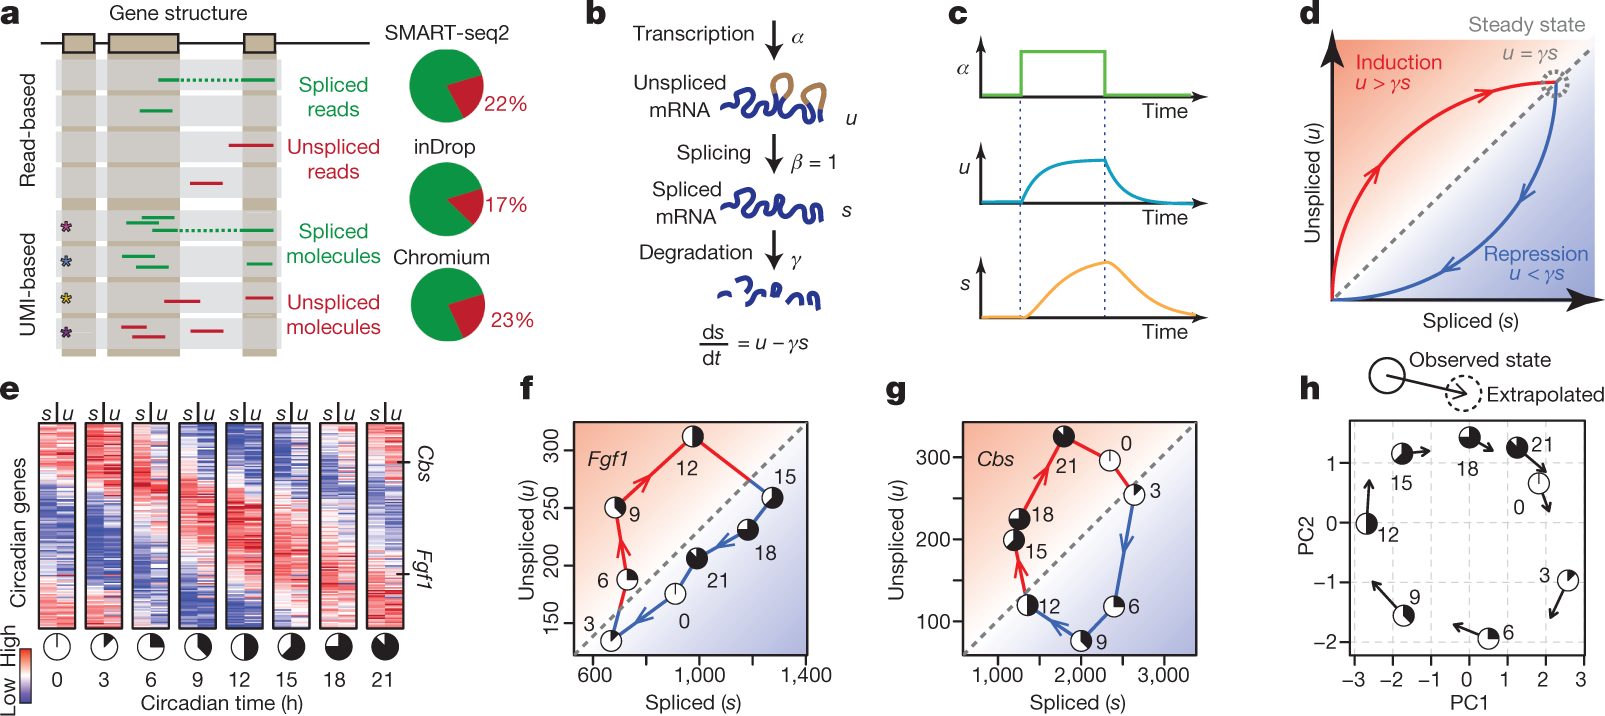
\includegraphics[width=0.8\textwidth]{figures/velocityFig1.png} 
%	\end{center}
%	\blfootnote{Image taken from \cite{pmid30089906}}
%	\end{frame}
%
%\begin{frame}{RNA Velocity}
%	\begin{itemize}
%		\item RNA Velocity is defined as the rate of change in spliced RNA with time
%		\item We obtain a value for each gene in each sample
%		\item Use dimensional reduction techniques $\implies$ project a velocity field onto clusters
%	\end{itemize}
%\end{frame}
%
%\begin{frame}{RNA Velocity}
%	\begin{center}
%	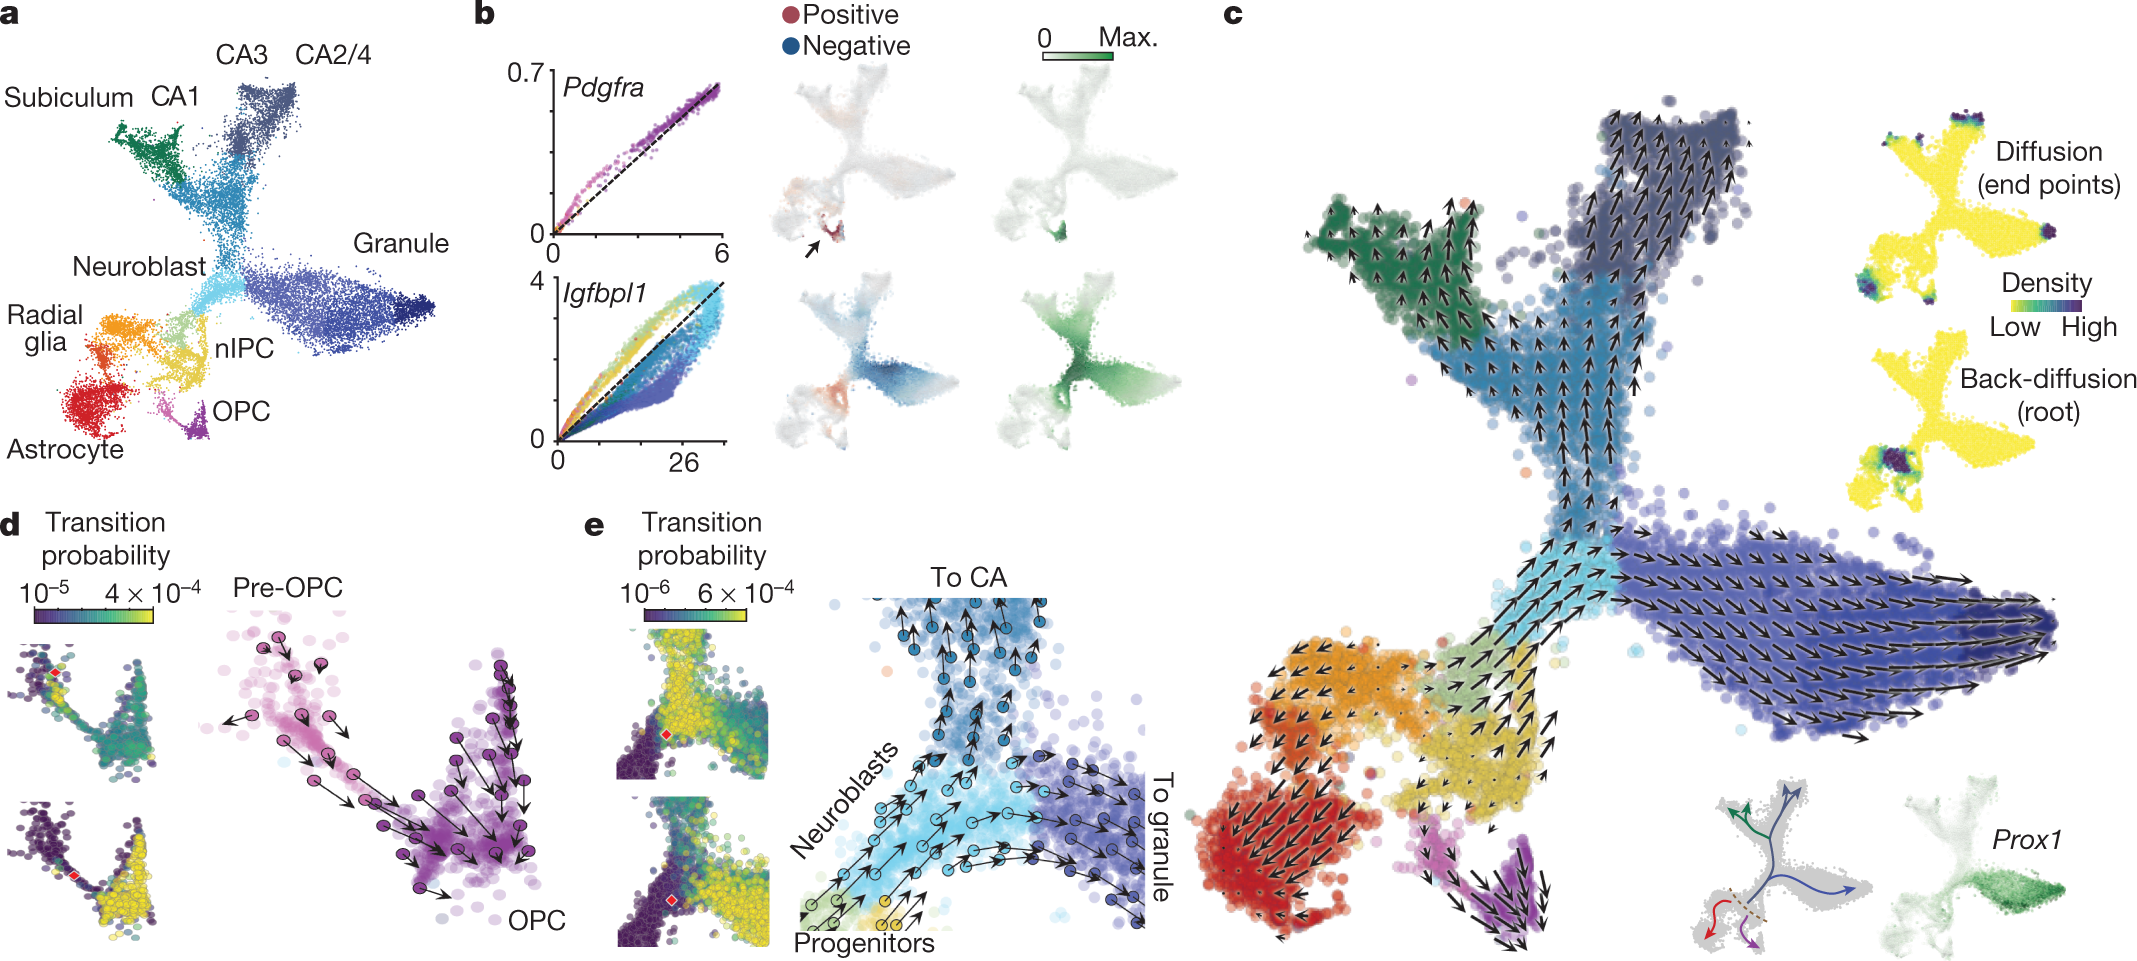
\includegraphics[width=0.8\textwidth]{figures/velocityFig3.png} 
%	\end{center}
%	\blfootnote{Image taken from \cite{pmid30089906}}
%\end{frame}

\end{document}
